\documentclass[a4paper,11pt]{scrartcl}

\usepackage[utf8]{inputenc}
\usepackage[ngerman]{babel}
\usepackage[T1]{fontenc}
\usepackage{amsmath}
\usepackage{graphicx}
\usepackage{tabularx}
\usepackage[a4paper, left=2cm, right=2cm, top=2.8cm, bottom=2.8cm]{geometry}
\usepackage{tikz}   
\usepackage[scaled]{helvet}
\usepackage{tabto} 
\usepackage{fancyhdr}
\usepackage{multirow}

\renewcommand*{\familydefault}{\sfdefault}

\pagestyle{fancy}

\setkomafont{section}{\huge}
\setkomafont{subsection}{\Large}


\lhead{Maximilian Hoffmann}
\chead{Betrieblicher Auftrag \\ \textbf{Kabeltester}}
\rhead{
\includegraphics[width=3cm]{Bilder/BMK_LOGO.png}}

%%%%%%%%%%%%%%%%%%%%%%%%%%%%%%%%%%%%%%%%%%%%%%%%%%%%%%%%%%%%%%%%%%%%%%%%%%%%%%%%%%%%%%%%%%%%%%%%%%%%%%%%%%%%%%%%%%%%%%%%%%%%%%%%%%%%%%%%%%%%%%%																																			 %
%														Funktionen der Schaltung															%
%																																		     %
%%%%%%%%%%%%%%%%%%%%%%%%%%%%%%%%%%%%%%%%%%%%%%%%%%%%%%%%%%%%%%%%%%%%%%%%%%%%%%%%%%%%%%%%%%%%%%%%%%%%%%%%%%%%%%%%%%%%%%%%%%%%%%%%%%%%%%%%%%%%%%

\begin{document}

%%%%%%%%%%%%%%%%%%%%%%%%%%%%%%%%%%%%%%%%%%%%%%%%%%%%%%%%%%%%%%%%%%%%%%%%%%%%%%%%%%%%%%%%%%%%%%%%%%%%%%%%%%%%%%%%%%%%%%%%%																																						%
%														Versorgung														%
%																														%
%%%%%%%%%%%%%%%%%%%%%%%%%%%%%%%%%%%%%%%%%%%%%%%%%%%%%%%%%%%%%%%%%%%%%%%%%%%%%%%%%%%%%%%%%%%%%%%%%%%%%%%%%%%%%%%%%%%%%%%%%

\section{Schaltplanentwurf}

\begin{center}
In diesem Teilbereich der Dokumentation, wird auf die Funktion der Schaltung eingegangen. 
\end{center}

\subsection{Versorgung}

\subsubsection{Schutzbeschaltung}

\begin{center}
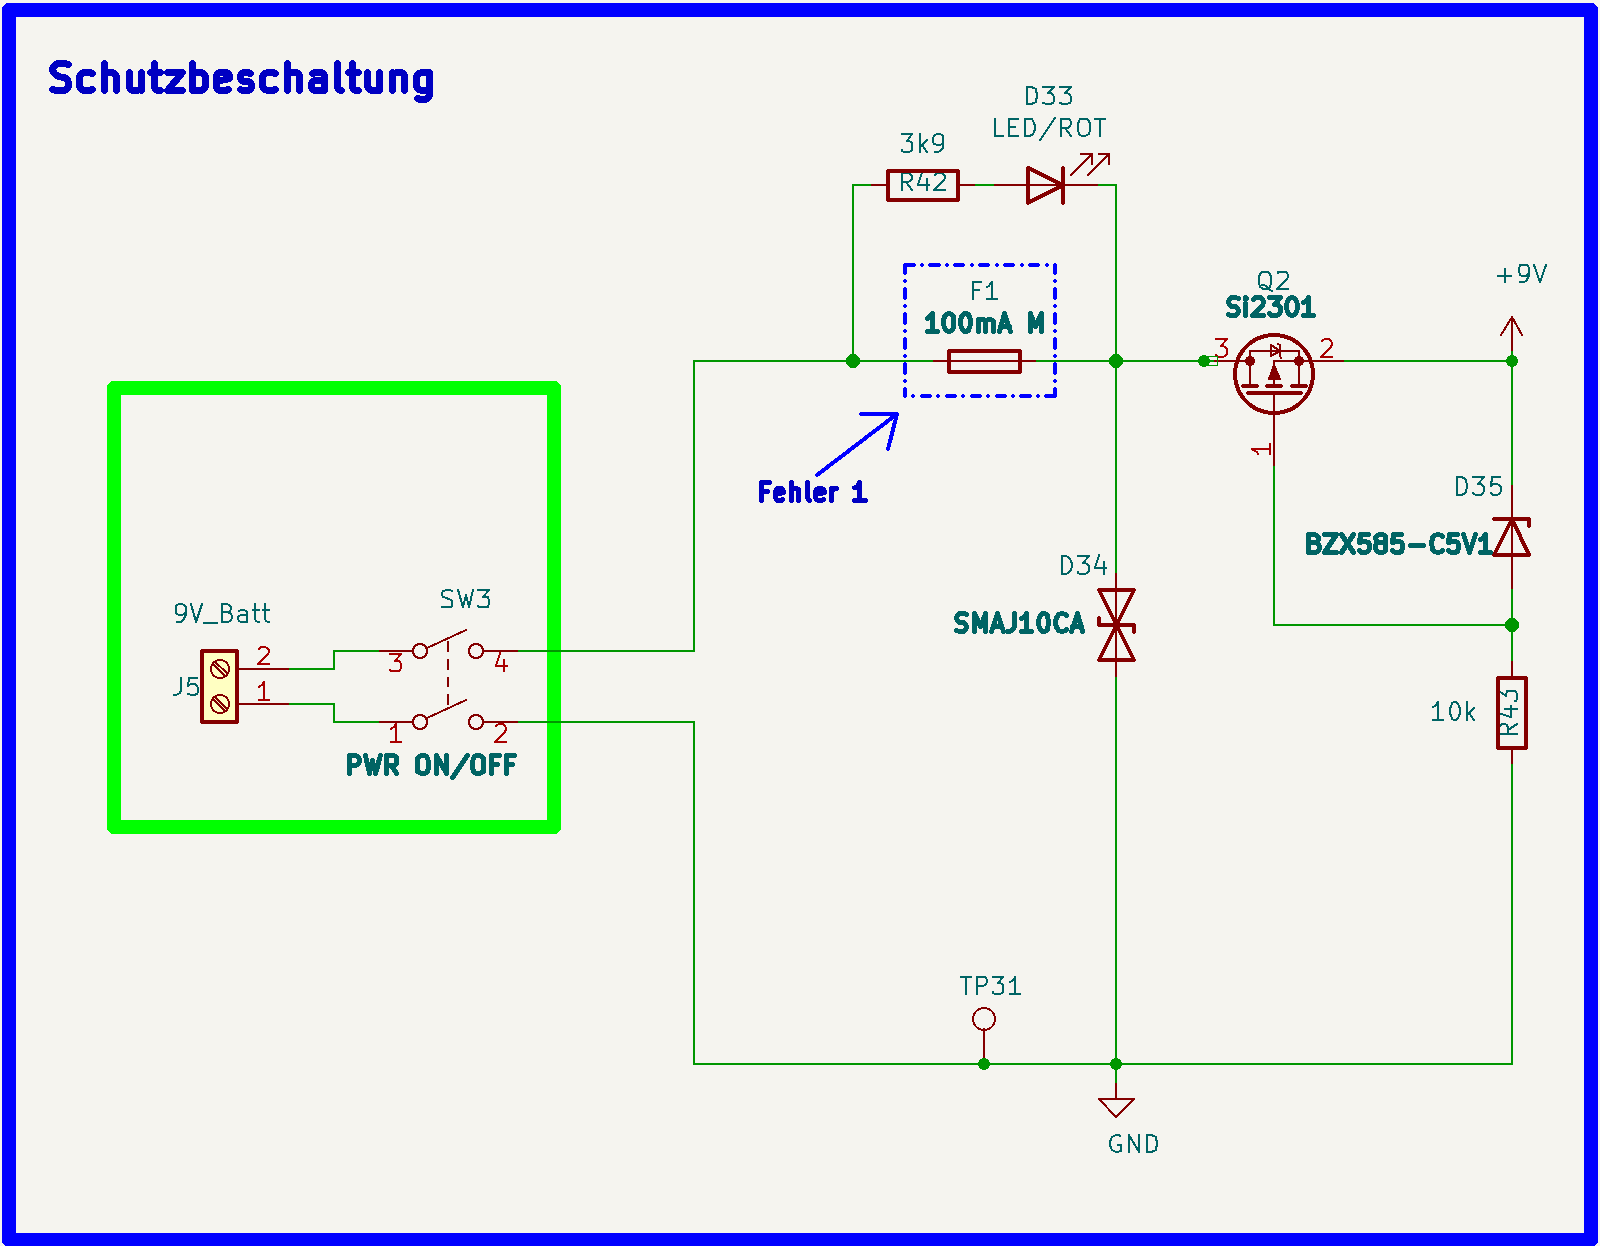
\includegraphics[width=10cm]{Bilder/Schutzbeschaltung.png}
\end{center}

Um die Schaltung zu schützen, wurde auf eine umfangreiche Eingangsschutzbeschaltung gesetzt. Die Versorgungsspannung kann dabei zweipolig durch den Schalter \glqq Power ON/OFF SW3 \grqq{} abgeschaltet werden.
\\
\\
Die mittelträge Sicherung F1 ist für den Überstromschutz verantwortlich. Löst diese aus, so bildet sich ein Strompfad über R42 und D33, welcher den Strom auf ein Maximum von 2mA in der gesamten Schaltung begrenzt. Als Ergebnis wird D33 rot leuchten. Im Normalbetrieb wird der Strompfad R42 - D33 durch den ohmschen Widerstand der Sicherung F1 (12R) überbrückt.
\\
\\
Um den Eingang des DC/DC Wandlers vor Überspannungsspitzen zu schützen wurde auf eine 10V TVS Diode gesetzt. Die Eingangsspannung dieser Schaltung wird dadurch auf ein Spannungsmaximum von 10V begrenzt. 
\\
\\
Da es bei einer Batterieanwendung sehr schnell zu einer ungewollten Verpolung der Anschlüsse kommen kann, ist ein umfangreicher Verpolungsschutz Pflicht. Liegt eine korrekt gepolte Spannung an, so bildet sich ein Strompfad über die Z-Diode D35 und den strombegrenzenden Widerstand R43. Die über die Z-Diode abfallende Spannung von 5,1V liegt somit auch an den Anschlüssen \glqq Source und Gate \grqq{} des P-Channel MOSFET Q2 an. Die Vorgabe für eine leitende Drain - Source Strecke eines P-Channel MOSFET ist ein um ca. 5V positiveres Potential an Source gegenüber Gate. Im korrekt gepolten Fall lässt sich dieser Zustand darauf zurückführen.
\\ 
Im Falle einer Verpolung bildet sich ebenfalls der Strompfad (D35 und R43). Durch die umgekehrte Polung ist nun D35 nicht mehr als Z-Diode, sonder als normale Si-Diode zu betrachten. Somit ist das Potential an Gate um die \glqq Forward Spannung \grqq{} von D35 positiver als Source.  Der P-Channel MOSFET sperrt und ein Stromfluss wird unterbunden.
\\
\\
\subsubsection{DC/DC Wandler}

\begin{center}
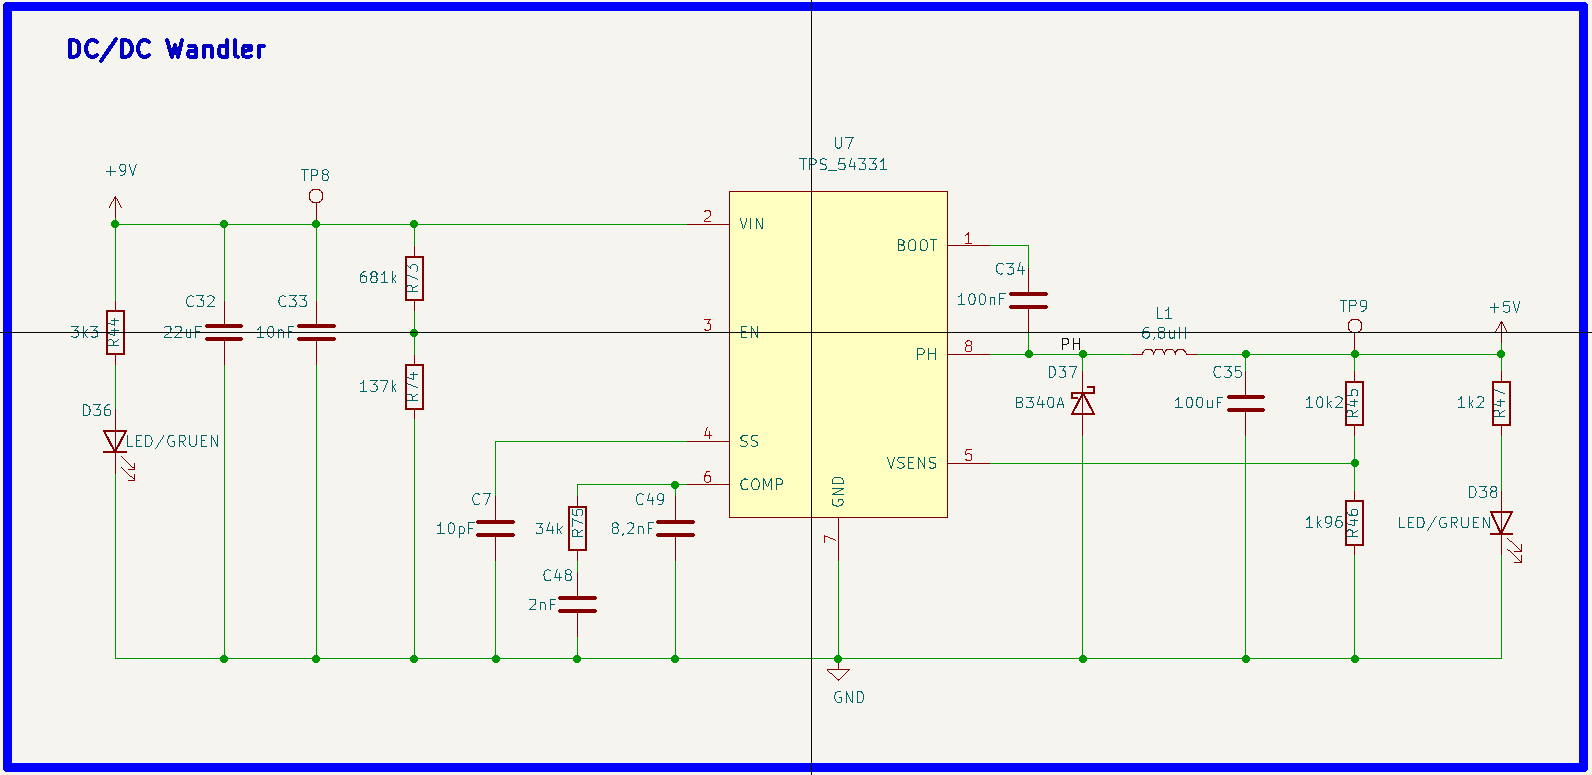
\includegraphics[width=16cm]{Bilder/DCDCWandler.png}
\end{center}

Bei der Auswahl des DC/DC Wandlers wurde auf die Verfügbarkeit bei BMK im Haus geachtet. Die Dimensionierung der externen Bauelemente wurde mit Hilfe des \glqq Texas Instruments Power Designer \grqq{} durchgeführt. Die grünen LED's D36 und D38 sorgen für ein optisches Feedback der Spannungen. Allgemein wurde der Wandler für eine Ausgangsspannung von +5V und einen Ausgangsstrom von ca. 1,5A dimensioniert. Mit den Widerständen R73 und R74 kann der Schaltregler bei Über/-Unterspannung abschalten. Die obere Schwellwertspannung beträgt +10V. Die untere Schwellwertspannung beträgt +8V.

\begin{center}
\begin{align}
	R73 &= \dfrac{V_{\Delta}}{3uA} = \dfrac{2V}{3uA} = 666k  \Rightarrow 680k\\
	R74 &= \dfrac{1,25V}{\dfrac{Vs - 1,25V}{R73} + 1uA} = \dfrac{1,25V}{\dfrac{8V - 1,25V}{680k} + 1uA} = 126k \Rightarrow 150k	\\
	V_{OUT}	&= V_{REF} + (\dfrac{R45}{R46} + 1) = 0,8V + (\dfrac{10,2k}{1,96k} + 1) = 4,96V
\end{align}
\end{center}


\newpage

%%%%%%%%%%%%%%%%%%%%%%%%%%%%%%%%%%%%%%%%%%%%%%%%%%%%%%%%%%%%%%%%%%%%%%%%%%%%%%%%%%%%%%%%%%%%%%%%%%%%%%%%%%%%%%%%%%%%%%%%%																																						%
%														NE555 Taktgeber													%
%																														%
%%%%%%%%%%%%%%%%%%%%%%%%%%%%%%%%%%%%%%%%%%%%%%%%%%%%%%%%%%%%%%%%%%%%%%%%%%%%%%%%%%%%%%%%%%%%%%%%%%%%%%%%%%%%%%%%%%%%%%%%%

\subsection{NE555 Taktgeber}

\subsubsection{Takt}

\begin{center}
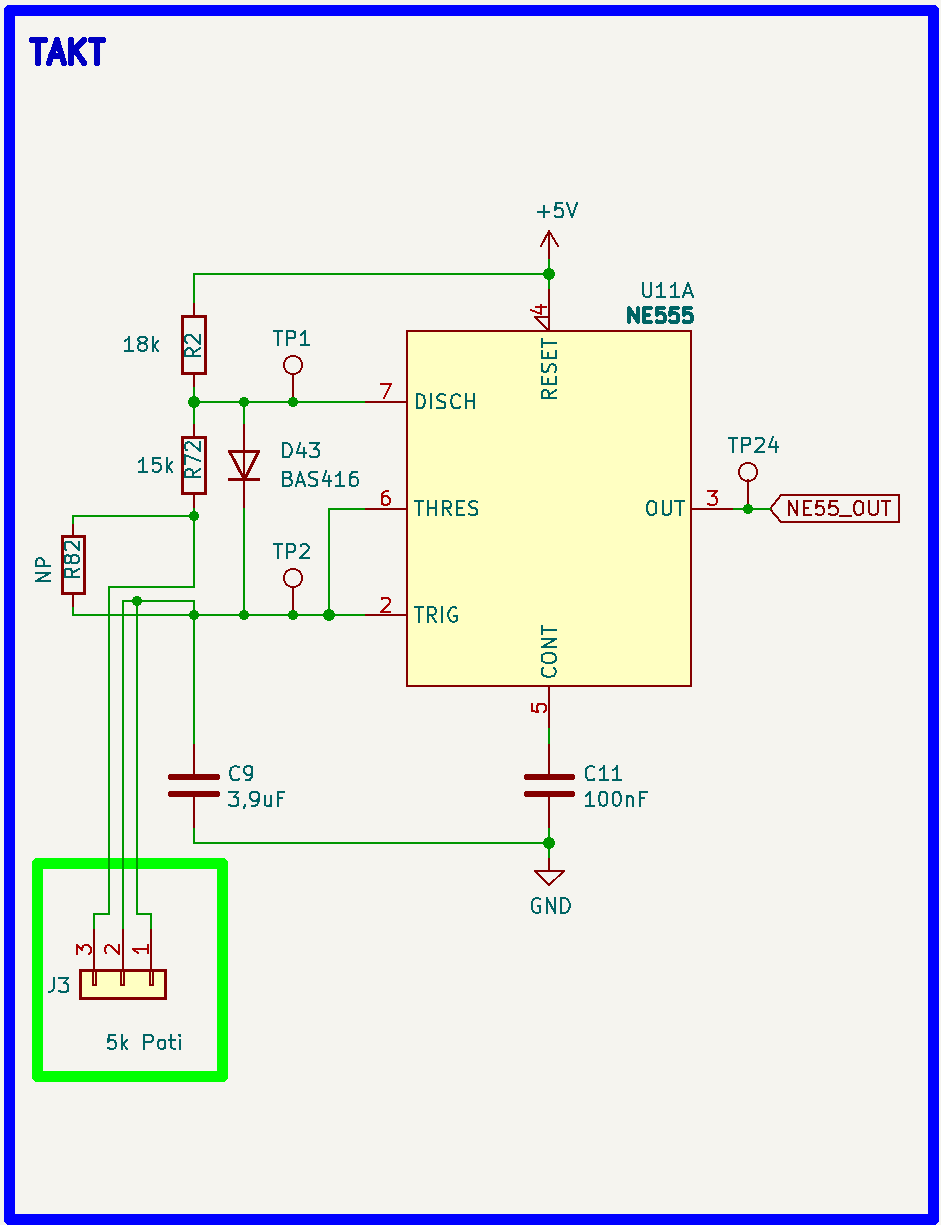
\includegraphics[width=10cm]{Bilder/Takt.png}
\end{center}

Als Taktgeber kommt der \glqq NE555 \grqq{} zum Einsatz. Dieser wird als astabile Kippstufe betrieben. Mit Hilfe der Diode D43 gleichen sich Impulszeit und Pausenzeit an. Über das Poti (Connector) J3 soll die Ausgangsfrequenz auf ca. 10Hz eingestellt werden können. 
\\
\\
Im Einschaltmoment ist C9 entladen. Liegt das Signal am Triggereingang unterhalb von $\frac{1}{3} VCC$, so wird das interne FlipFlop gesetzt. Der Ausgang (PIN 3) erfährt einen High-Pegel. Der Kondensator C9 lädt sich nun über den Strompfad R2 und D43 auf. Der Ladevorgang hält so lange an, bis das Spannungspotential an Pin 6 (Threshold) einen höheren Wert als $\frac{2}{3} VCC$ aufweist. Das bewirkt ein Rücksetzen des FlipFlop's und das entladen von C9 über R72 und den nun \glqq mit GND verbundenen\grqq{} Pin 7 (Discharge). Hat sich der Kondensator auf ein Spannungspotential unterhalb der $\frac{1}{3} VCC-Spannung$ entladen wird er Ausgang wider gesetzt und der Entladevorgang über Pin7 unterbunden. Dieser Vorgang wiederholt sich solange Energie von außen hinzugefügt wird. 

\begin{center}
\begin{align}
	f_{OUT} &= \dfrac{1}{0,69*R2*C9 + 0,69*(R72+R_{J3})* C9} = \dfrac{1}{0,69*18k*3,9uF*2} = 10,3Hz
\end{align} 
\end{center}

\newpage
\subsubsection{Taktumschaltung}

\begin{center}
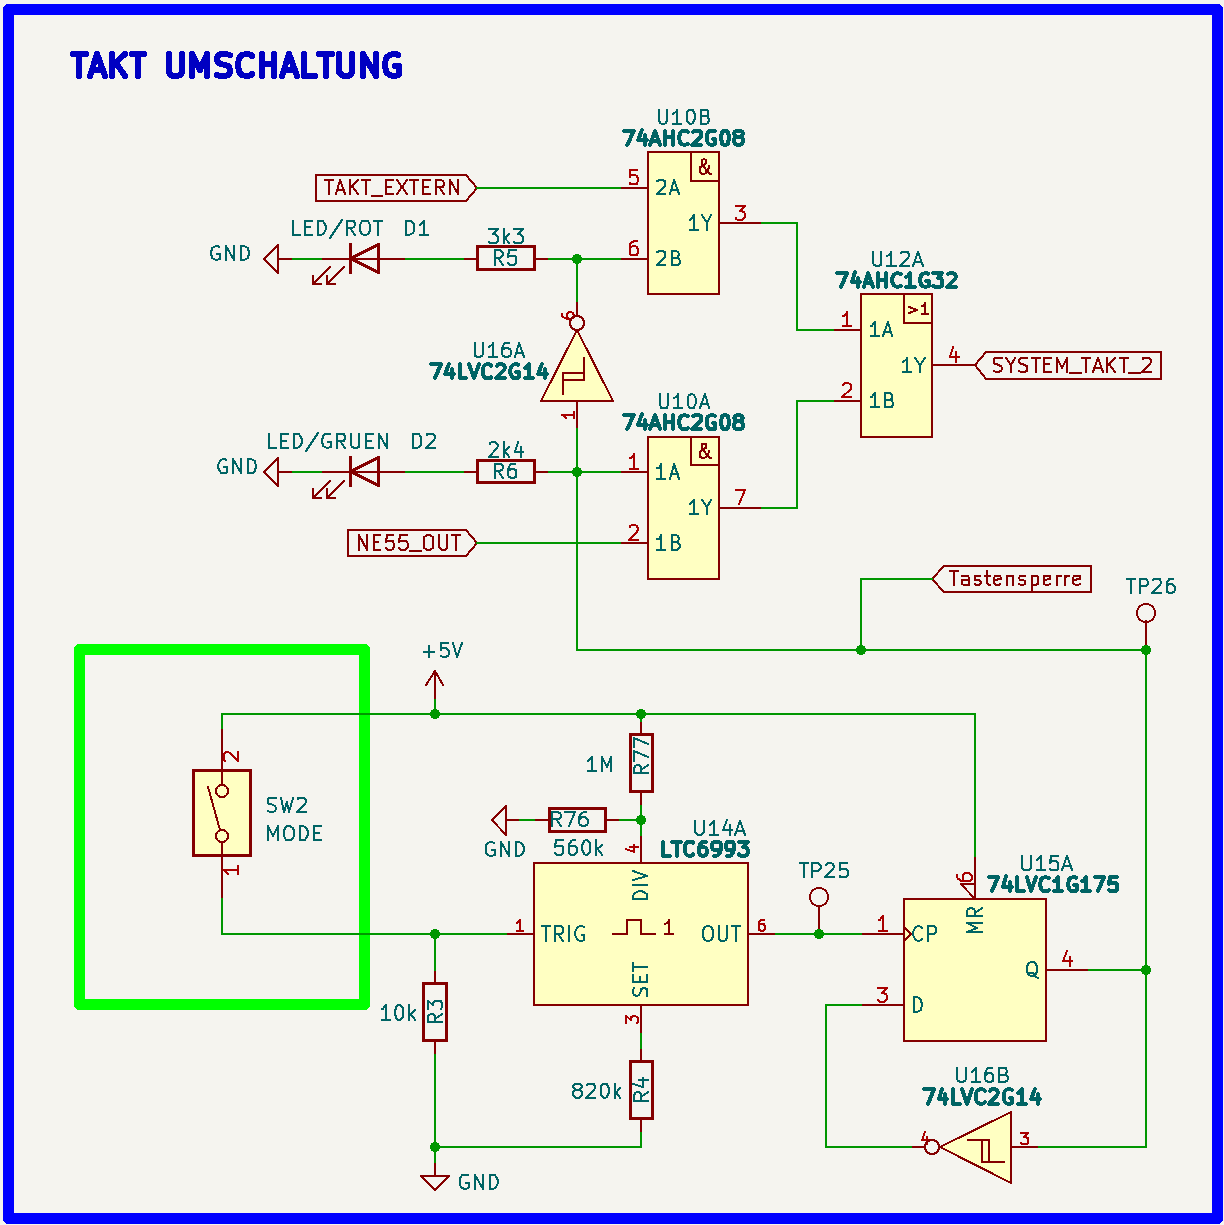
\includegraphics[width=13cm]{Bilder/Taktumschaltung.png}
\end{center}


\textbf{Funktionsbeschreibung LTC6993 U14}
\\
Das IC „LTC6993“ ist eine Monostabile Kippstufe mit einer einstellbaren Pulsweite von 1us – 33,6s. Dabei wird bei einem Impuls an dem Trigger-Eingang der Ausgang für eine einstellbare Zeit gespeichert bevor der Ausgang wieder in den stabilen Zustand zurück kippt. Über die Außenbeschaltung der Pin’s „DIV“ und „SET“ kann die Pulsweite (Kipp-Zeit) konfiguriert werden. Der Pin „DIV“ ist dabei intern mit einem 4 Bit A/D-Wandler beschalten. Dieser führt drei seiner Datenleitungen einem Taktteiler zu. Dieser Taktteiler ist dadurch zwischen 1 und 2 097 152 einstellbar. Die vierte Datenleitung (MSB) übergibt ihren Zustand dem Block „Output Polarity“. Dieser bestimmt den stabilen Ausgangspegel des Monoflops. Ein Widerstand zwischen GND und dem Pin „SET“ ist dabei für die Oszillator-Frequenz zuständig. Die Spannung zwischen „SET“ und GND wird dabei konstant auf 1V gehalten, was einen konstanten Stromfluss hervorruft. Die dabei möglichen Widerstandswerte liegen zwischen 50k und 800k (1,25uA-20uA), was einem Frequenzbereich von 1Mhz bis 62,5kHz entspricht. Die durch den Taktteiler geteilte Oszillatorfrequenz, setzt dabei ein RS-FlipFlop periodisch zurück. Ein Impuls am Trigger-Eingang setzt das FlipFlop, so dass es erst nach einer bestimmten Kipp-Zeit zurückgesetzt werden kann. Der FlipFlop-Ausgang ist dabei über den „Output Polarity“ Block mit dem Ausgang des IC‘s verbunden.

\newpage

\textbf{Funktion}
\\
Der Schaltungsteil \glqq Taktumschaltung \grqq{} ist für das Umschalten der zwei Taktquellen verantwortlich. Es kann zwischen den intern (durch den NE555 generierten) Takt und den durch eine vorgeschaltene Messplatine extern zugeführten Takt umgeschaltet werden. Ausschlaggebend dafür sind zwei Schaltungsteile. Durch betätigen des Tasters SW2 (MODE) soll zwischen den Taktquellen umgeschaltet werden. Da jede Tasterbetätigung ein mechanisch verursachtes prellen der Kontakte verursacht, muss dies durch das nachgeschaltete  Monoflop U14 unterbunden werden. Die Zeit, die das Monoflop benötigt mit seinem Ausgang auf einen eingangsseitigen Triggerimpuls zu reagieren, sollte länger benötigen als das prellende Signal selbst. Somit kann am Ausgang von U14 eine saubere Signalflanke zustande kommen. 
\\
Das nachgeschaltete D-FlipFlop ist in seiner Verschaltung, mit auf den Dateneingang zurückgeführten invertierten Ausgang, als Toggle FlipFlop zu betrachten. Für einen Pegelwechsel am Ausgang Q des T-FlipFlop ist eine steigende und fallende Flanke notwendig. Eine Betätigung mit zwei dynamischen Flanken verursacht demnach einen Pegelwechsel an TP28 mit nur einer dynamischen Flanke. 
\\
Die auf TP28 folgende Schaltung ist als zweifach TOR-Schaltung mit nur einen Steuereingang zu verstehen. Ein High-Signal an TP28 bedeutet für das UND-Gatter U10B eine durch die Invertierung verursachte Sperrung des externen Signales. Das UND-Gatter U10A kann nun den digitalen Signalverlauf des globalen Label's \glqq NE55 OUT \grqq{} auf seinen Ausgang übertragen. Bei einem Low-Pegel sind die geschilderten Zustände vertauscht. Da einer der beiden UND-Gatter immer einen Low-Pegel an seinem Ausgang vor zu weißen hat, wird das Signal an den Eingang des ODER-Gatter U12A einfach auf den Ausgang übertragen und über das globale Label im Schaltplan globalisiert.

\subsubsection{Taktteilung}

\begin{center}
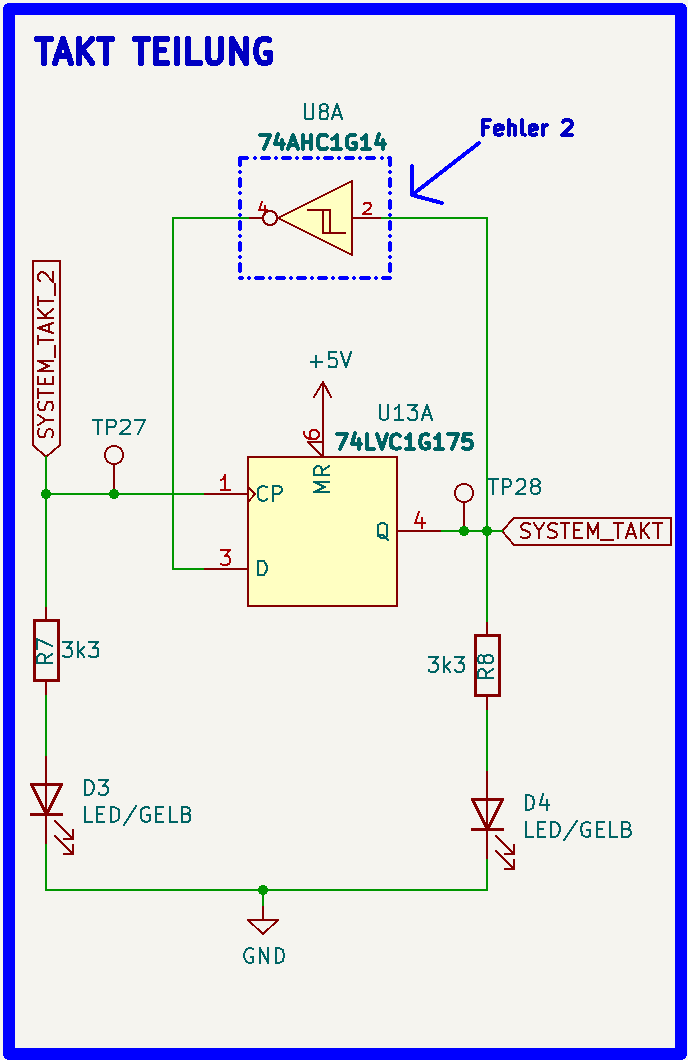
\includegraphics[width=7cm]{Bilder/Taktteilung.png}
\end{center}

Für einen folgenden Schaltungsteil wird ein Takt, welcher die doppelte Frequenz des Messtaktes besitzt benötigt. Die in meinen Augen einfachste Lösung für dieses Problem, ist die Taktteilung des Timer NE555 Taktes. Der geteilte Takt wird dabei als Grundtakt verwendet und der durch den NE555 generierte Takt wird in dem folgenden Schaltungsteil Anwendung finden.

\newpage

\subsection{Dezimal Zähler}

\subsubsection{Messung Starten}

\begin{center}
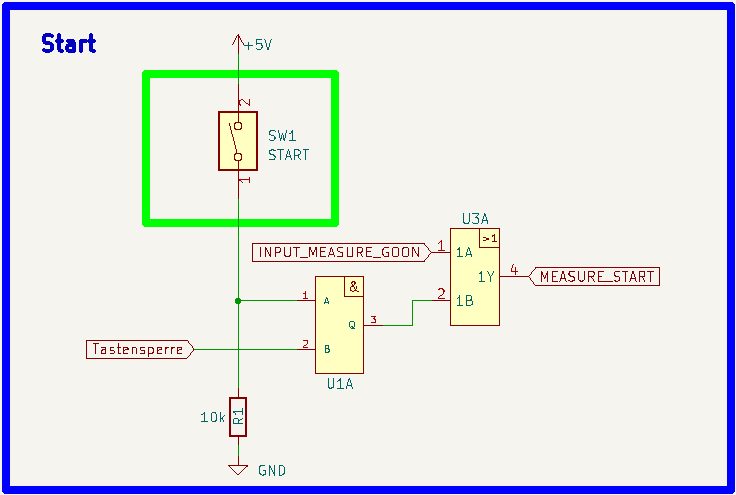
\includegraphics[width=12cm]{Bilder/Start.png}
\end{center}

Die Messung kann über Betätigung des Tasters SW1 (START) oder über ein externes Signal (Label: INPUT MEASURE GOON) gestartet werden. Befindet sich die Messplatine im \glqq Master Mode \grqq{} (\textbf{Master Mode:}  Interner Takt \textbf{Slave Mode:} Externer Takt), so führt eine Betätigung des Tasters SW1 zum Start der Messung.  Befindet sich die Messplatine im \glqq Slave Mode \grqq{} so kann nur durch ein externes Signal die Messung gestartet werden.


\subsubsection{Reset}

\begin{center}
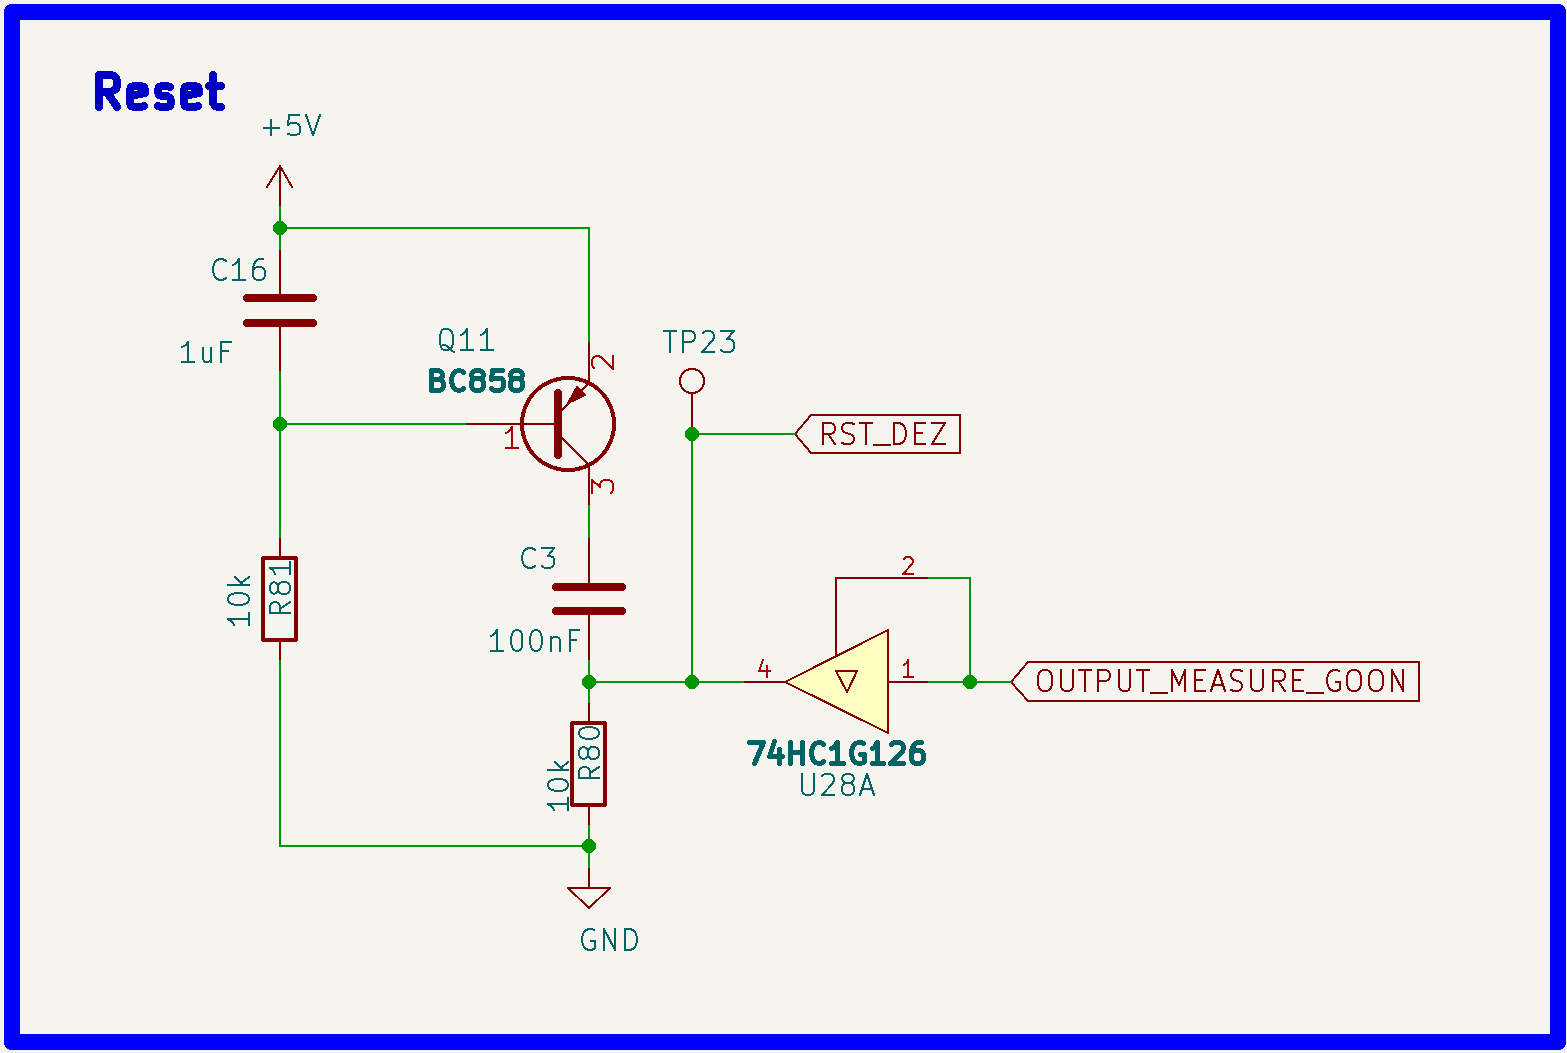
\includegraphics[width=12cm]{Bilder/Reset.png}
\end{center}

Die Aufgabe der folgenden Schaltung liegt darin kurze Zeit nach dem Einschalten, die FlipFlop's bestehend aus \textbf{FF1:} U2A und U2B \textbf{FF2:} U2C und U2D in einen bestimmten Ausgangszustand zu setzen. Dies ist von entscheidender Bedeutung für die Funktion der Schaltung. 
\\
\\
Im Einschaltmoment bildet sich ein Strompfad über C16 und R81. C16 liegt dabei parallel zu den Anschlüssen \glqq Emitter und Basis\grqq{} des PNP-Transistors Q11. Da im Einschaltmoment sich zwischen den Kondensatorplatten noch kein elektrisches Feld aufgebaut hat, liegen Emitter und Basis auf dem selben Potential. Ein Stromfluss ist daher nicht möglich und der Transistor Q11 sperrt. C16 beginnt sich über die Zeit langsam aufzuladen. Hat sich ein bestimmtes Spannungspotetial über C16 aufgebaut (ca. 0,7V $U_{BE}$) so ist ein Stromfluss aus der Basis hinaus möglich. Nach einer bestimmten Verzögerung ist nun auch ein Stromfluss im zweiten Strompfad (Q11 - C5 - R80) möglich. Das noch nicht vorhandene Spannungspotential über C3 führt zu einem anfänglichen 5V Pegel über R80 und somit auch am globalen Label \glqq RST DEZ \grqq{}. Dieser Pegel verkleinert sich über die Zeit immer mehr, da sich nun auch über C3 ein Spannungspotential bildet. 
\\
Das IC U28A dient zur Stromkreisentkopplung und soll beim Resetvorgang einen Kurzschluss vermeiden.

\subsubsection{Controlling}

\begin{center}
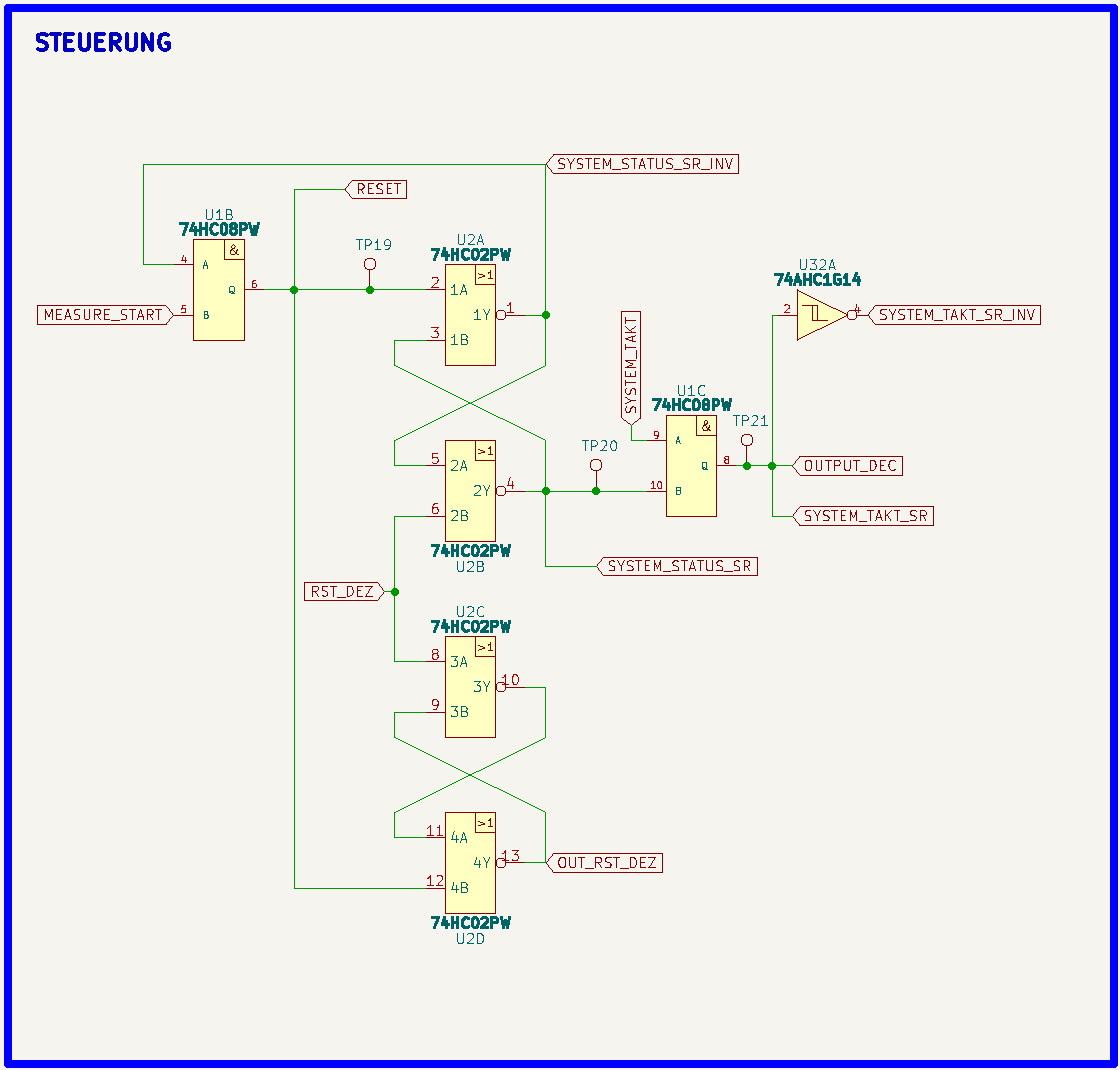
\includegraphics[width=12cm]{Bilder/Controlling.png}
\end{center}

Durch die voran gegangene Schaltung, welche die FlipFlops \textbf{FF1:} U2A und U2B \textbf{FF2:} U2C und U2D in die richtigen Ausgangszustände bringt, kann nun ein einwandfreier Start der Messung durchgeführt werden. 
\\
\\
Zum Starten der Messung befindet sich an Pin 4 des UND-Gatters U1B ein High-Pegle. Ein High-Pegel an Pin 5 U1B führt dann zu einem Rücksetzen des FlipFlops \textbf{FF1}. Durch das Wechseln der Ausgangszustände, liegt nach einer Verzögerung (Abhängig von der Gatterlaufzeit des \textbf{FF1}) ein Low-Pegel an. Ein sich ständig an Pin 5 (U1B) änderndes Signal, verursacht durch das mechanische prellen des Tasters SW1 (START), wird somit durch das TOR-Gatter U1B nach kurzer Zeit unterdrückt.
\\
Das High-Signal an PIN 10 (U1C) 


\end{document}